\documentclass{article}

% Language setting
% Replace `english' with e.g. `spanish' to change the document language
\usepackage[english,russian]{babel}
\usepackage{amsmath}

%графика
\usepackage{wrapfig}
\usepackage{graphicx}
\usepackage{pgfplots}
\usepackage{tikz}


\usepackage{tcolorbox}

% Set page size and margins
% Replace `letterpaper' with `a4paper' for UK/EU standard size
\usepackage[letterpaper,top=2cm,bottom=2cm,left=3cm,right=3cm,marginparwidth=1.75cm]{geometry}

% Useful packages
\usepackage{amsmath}
\usepackage{amssymb}
\usepackage{graphicx}
\usepackage{fixltx2e}
\usepackage[colorlinks=true, allcolors=blue]{hyperref}

\usepackage{geometry}
\geometry{left=25mm,right=25mm,
 top=25mm,bottom=25mm}

\title{Quantitative Analytics.\\
Lectures. Weeks 5 - 8. \\
Swaps. \\
Свопы.}
\author{Dmitry Sereda}

% Колонтитулы
\usepackage{fancyhdr}
\pagestyle{fancy}
\renewcommand{\headrulewidth}{0.1mm}  
\renewcommand{\footrulewidth}{0.1mm}
\lfoot{}
\rfoot{\thepage}
\cfoot{}
\rhead{CMF-2022}
\chead{}

\begin{document}
\maketitle

% Оглавление
\setcounter{tocdepth}{1} % {2} - в оглавлении участвуют chapter, section и subsection. {1} - только chapter и section
\renewcommand\contentsname{Оглавление}
\tableofcontents
\newpage

% \section{Dictionary, Definitions, Abbreviations}

% \subsection{Dictionary}
% \begin{itemize}
%     \item IR - Interest rate - процентная ставка.
%     \item Compounding - платежи (idk)
% \end{itemize}

% \subsection{Definitions and Abbreviations}
% \begin{itemize}
%     \item SAR - Stated annual rate.
%     \item EAR - Effective annual rate.
%     \item FoC - Frequency of Compounding
%     \item PMT - Payment
%     \item r - Interest rate (at the moment). 
% \end{itemize}

\renewcommand{\labelitemi}{\tiny$\bullet$}
\renewcommand{\figurename}{Fig.}

 \section{Определение ванильного свопа}
 \textbf {Vanilla Interest Rate Swap} - простейший вид свопа, деривативный контракт, по которому одна сторона соглашается платить другой стороне периодический фиксированный процент на номинал в течение срока жизни данного контракта, в то время как другая сторона, в свою очередь, соглашается платить первой стороне периодический переменный процент на этот же номинал. Все платежи проводятся в одной валюте, поэтому обмен номиналами в конце не проводится.

\begin{figure}[h]
\centering
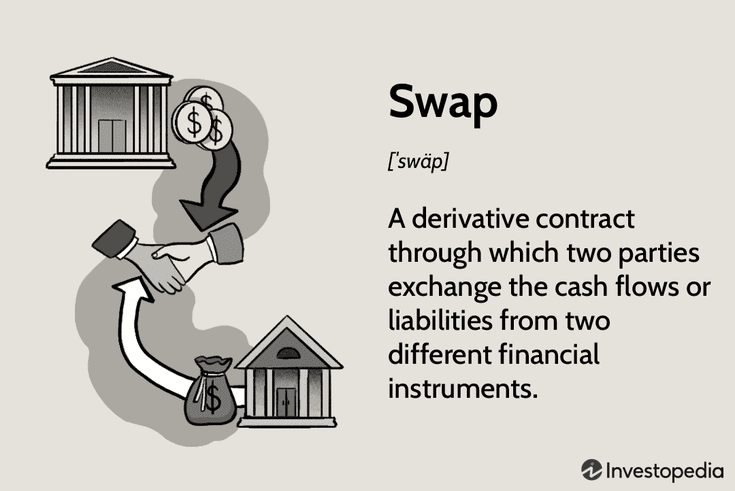
\includegraphics[width=0.7\textwidth]{swap definition.png}
\label{loadings}
\end{figure}

\begin{itemize}
     \item В общем случае не обязательно, чтобы платежи были в одной валюте, а также обе "ноги" могут быть как фиксированные, так и переменные.

     \item Довольно часто в качестве переменного процента используется значение LIBOR (London Interbank Offer Rate)
 \end{itemize}


\section{Денежные потоки ванильного свопа}

\begin{figure}[h]
\centering
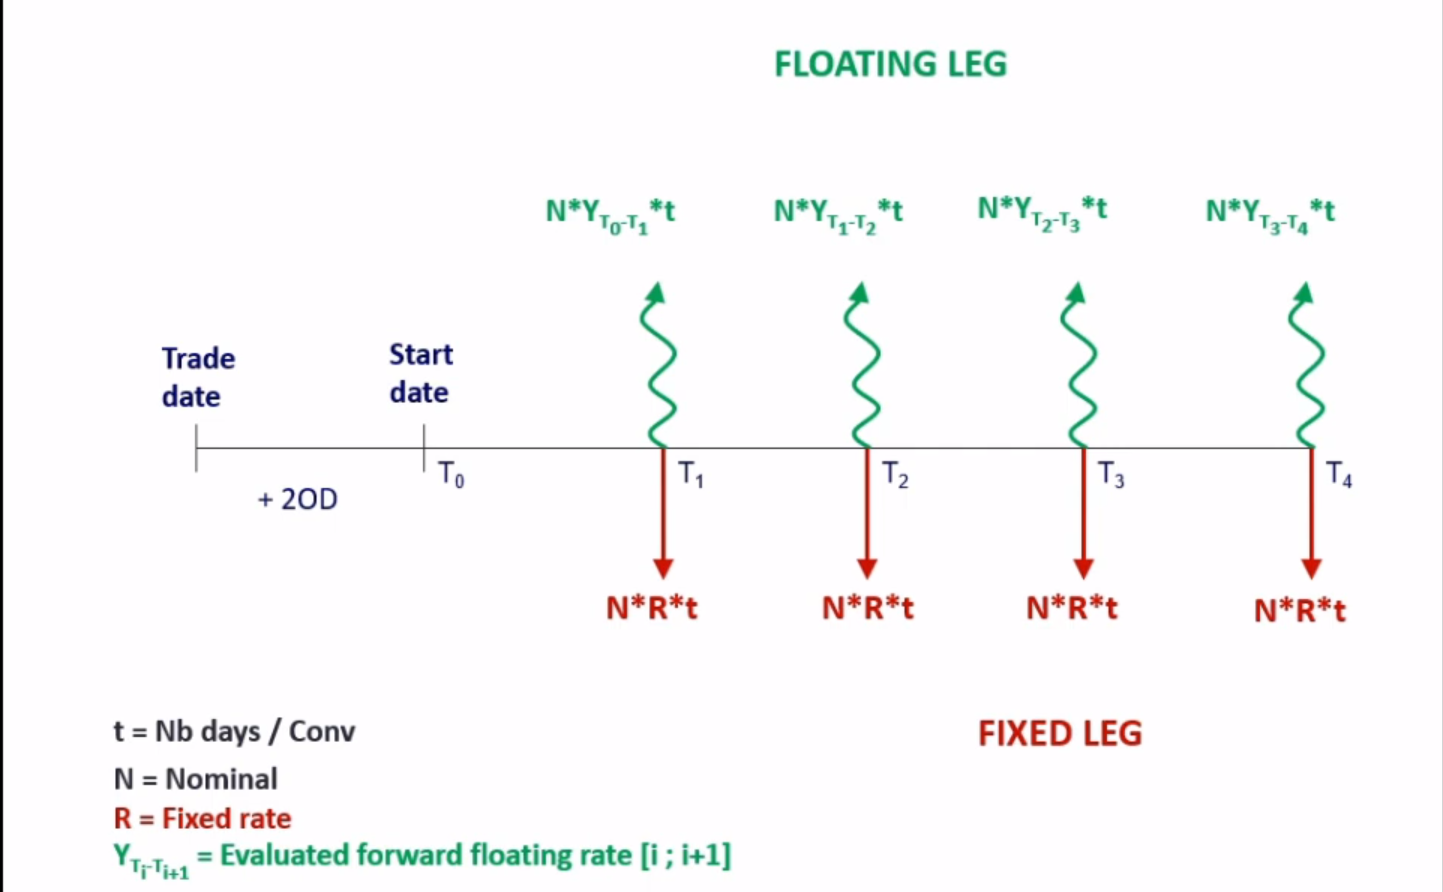
\includegraphics[width=0.6\textwidth]{swap cash flows.png}
\label{loadings}
\end{figure}

\text {Вступая} в данный договор, вы обязуетесь как получать некоторую сумму денег, так и платить. Совокупность денежных потоков, направленных в одном направлении, называется нога (leg). 

\begin{itemize}
    \item Как было уже сказано ранее, ванильный своп имеет две ноги: фиксированную и переменную.

    \item В качестве переменного процента за данный период берётся значение бенчмарка (инструмента, привязанного к переменной ноге) за начало периода, если не сказано обратного.

    \item Платежи не обязательно должны выпадать на один и тот же день.
\end{itemize}

\section{Причины, по которым участники могут захотеть заключить своп-соглашение}

\text{}

\textbf{Сценарий 1:} Компания уже имеет некоторое обязательство с выплатой фиксированной ставки (например, после выпуска облигаций), но хочет выплачивать переменные платежи вместо фиксированных.

\textbf{Сценарий 2:} Часто в сделках такого рода принимают участие финансовые посредники, такие как банки, которые берут дополнительную комиссию за риск неисполнения обязательств сторонами. В случае неисполнения обязательств одной из сторон посредник обязуется выполнить обязательства для другой стороны.

\textbf{Сценарий 3:} В зависимости от кредитного рейтинга участники рынка могут получить займ под разные проценты. Так, например, компания А, которая является более надёжной в глазах кредиторов, может получить займ под 5\%. В то время как менее надёжная компания Б только под 6.5\%, что даёт нам спред(разницу) в 1.5\%. При работе же с переменными ставками эти компании могли бы получить займы под LIBOR + 0.1\% и LIBOR + 1\% соответсвенно, т.к. спред при работе с переменными ставками как правило меньше.

\section{Вычисление стоимости свопа}
\subsection{Подход, основанный на двух непрерывных бондах}

\textbf{Условие:}

Предположим, некоторое время назад было заключено соглашение, по которому финансовый субъект согласился получать 6-месячный LIBOR и платить 3\% годовых (начисление процентов происходит раз в полугодие) с номиналом в 100 миллионов \$. Оставшееся время жизни свопа составляет 1.25 года. Непрерывные процентные ставки LIBOR для 3, 9 и 15 месяцев равны, соответственно, 2.8\%, 3.2\% и 3.4\%. Процентная ставка 6-месячного LIBOR в последнюю дату платежа равна 2.9\% (с полугодовым начислением процентов).

\begin{figure}[h]
\centering
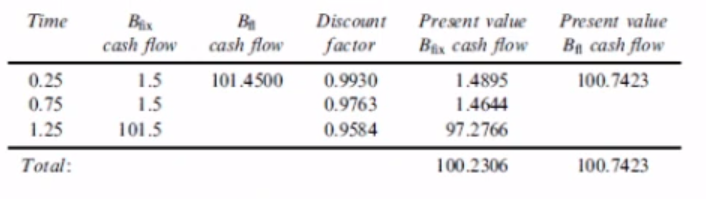
\includegraphics{bonds approach.png}
\label{loadings}
\end{figure}

\text{Денежные} потоки бонда с фиксированной ставкой равны 1.5, 1.5 и 101.5. Discount factors для этих потоков: $e^{-0.28*0.25}$, $e^{-0.32*0.75}$, $e^{-0.34*1.25}$. Сумма дисконтированных денежных потоков равна 100.2306.

\text{Для} бонда с плавающей ставкой мы имеем денежный поток через 3 месяца в размере: $B_{fl} = 100 mil * 0.5*0.029 = 101.45 mil$. И его дисконтированная стоимость равна 100.7423.

\text{Что} даёт нам итоговую стоимость свопа: $V = PV_{fl} - PV_{fix} = 100.7423 - 100.2306 = 0.5117 mil \$ $

\subsection{Подход, основанный на Forward Rate Agreements (FRA)}

\begin{itemize}
\itemДанный подход является более универсальным и чаще применяется на практике
\end{itemize}

\textbf{Условие:}

Предположим, некоторое время назад было заключено соглашение, по которому финансовый субъект согласился платить 6-месячный LIBOR и получать 6\% годовых (начисление процентов происходит раз в полугодие) с номиналом в 1 миллион \$. Оставшееся время жизни свопа составляет 15 месяцев. Непрерывные процентные ставки LIBOR для 3, 9 и 15 месяцев равны, соответственно, 5.4\%, 5.6\% и 5.8\%. Процентная ставка 6-месячного LIBOR в последнюю дату платежа равна 5\% .

\text{}

\text{Посчитаем} денежные потоки для плавающей ноги.

Денежный поток через 3 месяца равняется: 1000000 * 0.05 / 2 = 25000.

Для подсчёта дальнейших платежей нужно посчитать форвардные ставки по следующей формуле:

\text{}

\begin{center}

$R_{forward} = R_2 + T_1 *\frac{R_2 - R_1}{T_2 - T_1}$

\end{center}

\text{}

В таком случае форвардные ставки для последующих периодов равны (это непрерывные ставки):

$R_{2, forward} = 0.056 + 0.25*(0.056 - 0.054)/(0.75 - 0.25) = 0.057 = 5.7\%$

$R_{2, forward} = 0.058 + 0.75*(0.058 - 0.056)/(1.25 - 0.75) = 0.061 = 6.1\%$

\begin{figure}[h]
\centering
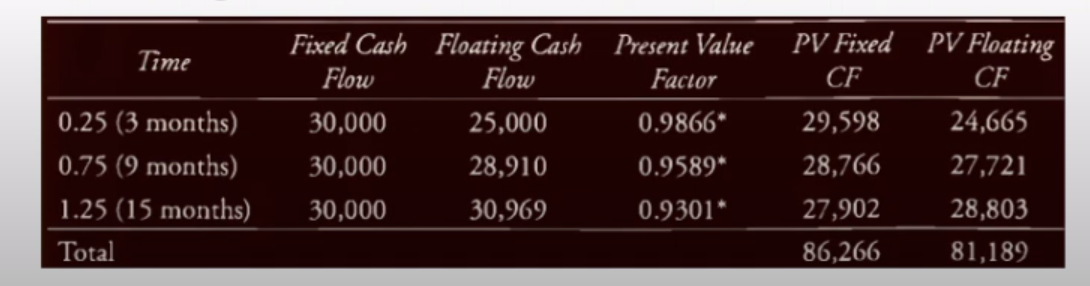
\includegraphics{fra approach.png}
\label{loadings}
\end{figure}

\text{}

\text{}
$V = PV_{fix} - PV_{fl} = 86266 - 81189 = 5077 \$ $

\section{Кредитный риск свопа}

\begin{itemize}
    \item Т.к. своп имеет зеркальную стоимость для разных сторон, то повышение стоимость свопа для одной стороны, означает понижение стоимости для другой стороны.
    \item Увеличение стоимости свопа приводит к увеличению кредитного риска.
    \item Тем не менее риск свопа значительно меньше риска бонда с тем же номиналом, т.к. стоимость свопа значительно меньше стоимости бонда.
\end{itemize}

\begin{figure}[h]
\centering
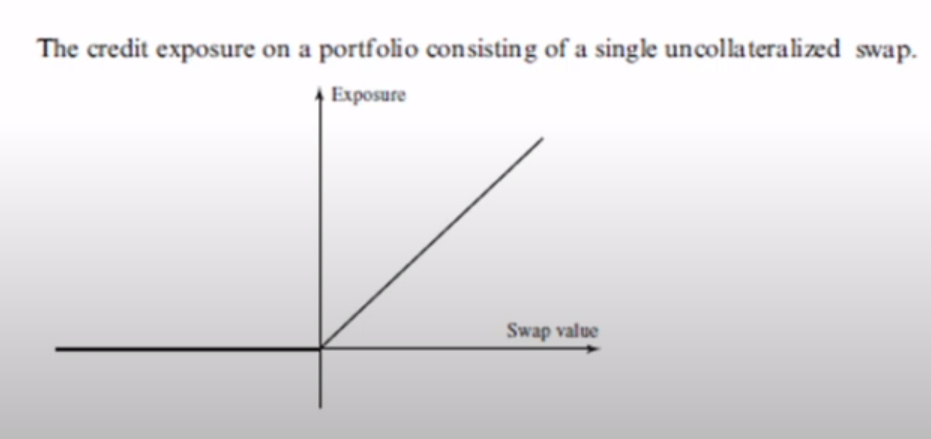
\includegraphics{credit risk.png}
\label{loadings}
\end{figure}

\newpage

\section{Другие виды свопов}
\subsection{Валютные свопы (Currency swaps)}

\begin{itemize}
    \item Обмен номиналами и процентными платежами в одной валюте за номинал и процентные платежи в другой
    \item Обмен платежами производится в начале и в конце контракта
    \item Используется для конвертации инвестиций/займов из одной валюты в другую
\end{itemize}

\subsection{Долевые свопы (Equity swaps)}
\begin{itemize}
    \item Одна сторона получает некие процентные платежи, а в обмен платит прибыль по некоторой акции/портфелю.
\end{itemize}

\subsection{Сырьевые свопы (Commodity swaps)}
\begin{itemize}
    \item Одна сторона получает фиксированные процентные платежи, а в обмен платит плавающую ставку в зависимости от стоимости сырья в контракте в течение срока его действия
    \item Такие контракты зачастую используются, чтобы хеджировать риски при покупке энергоресурсов.
\end{itemize}

\subsection{Свопы на волатильность (Volatility swaps)}
    \begin{itemize}
    \item Вид свопа, в рамках которого одна сторона платит фиксированные платежи, а другая в соответствие с исторической волатильностью за указанный период
    \end{itemize}

    
\end{document}